%%%%%%%%%%%%%%%%%%%%%%%%%%%%%%%%%%%%%%%%%%%%%%%%%%%%%%%%%%%%%%%%%%%%%%%%%%%%%
% Chapter 3: Modo de uso de genetics.js
%%%%%%%%%%%%%%%%%%%%%%%%%%%%%%%%%%%%%%%%%%%%%%%%%%%%%%%%%%%%%%%%%%%%%%%%%%%%%%%

%++++++++++++++++++++++++++++++++++++++++++++++++++++++++++++++++++++++++++++++

En este capítulo se expondrá una aplicación concreta implementada con \textbf{genetics.js}, la librería desarrollada. En esta implementación se ha construido una aplicación web usando React como framework de creación de interfaces de usuario, además de usar la librería para ejecutar un algoritmo evolutivo en el lado del cliente. \\

La intención que tiene este desarrollo es mostrar la capacidad de la que dispone la librería para ser ejecutada en el \textit{front-end}, junto a tecnologías modernas para la creación de páginas web. \\

\section{Descripción del problema a implementar}

La aplicación que se ha implementado es un simulador del problema de la mochila (\textit{Knapsack problem}), resuelto mediante un algoritmo evolutivo. La intención principal es que se puedan seleccionar la mayoría de parámetros posibles del algoritmo, para así poder ver como cambia el rendimiento con diferentes configuraciones de entrada. \\

Pero antes de describir el procedimiento concreto para desarrollar la aplicación, es importante realizar una definición del problema que se pretende abordar. Cabe destacar que el problema de la mochila es clásico en el ámbito de la optimización combinatoria \cite{karp1972reducibility}, y ha sido objeto de estudio desde el nacimiento del campo. \\

En la formulación del problema disponemos de $n$ items que pueden ser introducidos en la mochila. Cada item tiene dos atributos, su peso ($w_i$) y su valor o beneficio ($v_i$). De esta forma, la solución al problema trata de descubrir cual es el conjunto de items que debe introducirse en la mochila de tal forma que se maximize el beneficio total pero sin sobrepasar la capacidad ($W$) de la mochila. \\

De manera formal se puede describir el problema de esta forma:

\begin{equation*}
\begin{aligned}
& \underset{X}{\text{max}}
& & \sum_{i=1}^n v_i x_i \\
& \text{sujeto a}
& & \sum_{i=1}^n w_i x_i \leq W \\
&&& x_i \in \{0, 1\}
\end{aligned}
\end{equation*}

Donde $X = \{x_1, \dots, x_n\}$ es el conjunto de variables de decisión que establecen si el item $i$-esimo está o no presente en la mochila. \\

Existen múltiples técnicas para abordar este problema, incluso pudiendo ser resuelto mediante una técnicas exactas. Pero con motivo de probar la librería desarrollada, el problema se resolverá con un algoritmo genético. \\

La codificación que se utilizará para los individuos es la \textbf{codificación binaria}, donde cada uno de los genes del individuo representará si el ítem en la posición establecida se encuentra o no en la mochila. \\

Los parámetros del algoritmo que podrán seleccionarse serán:

\begin{itemize}
    \item \textbf{Tamaño de la población}: El tamaño de la población deberá estar comprendido entre 0 y 25. Donde el límite superior se ha establecido por criterios de claridad en la visualización.
    \item \textbf{Tipo de operador de cruce}: El operador de cruce que se puede seleccionar puede ser el crossover de un punto (\texttt{OnePointCrossover}), el crossover de n puntos (\texttt{NPointsCrossover}) o el crossover uniforme (\texttt{UniformCrossover}). Cabe destacar que dependiendo del operador elegido, se deberán establecer sus parámetros.
    \item \textbf{Método de selección de padres}: Se puede elegir entre \textit{roulette wheel} y \textit{stochastic universal sampling}.
    \item \textbf{Método de reemplazo}: Se puede seleccionar entre el remplazo basado en la edad (\texttt{AgeBasedReplacement}) y el basado en el fitness (\texttt{FitnessBasedReplacement}).
    \item \textbf{La tasa de mutación}: La tasa de mutación (\textit{mutation rate}), puede establecerse, teniendo 0.5 como valor por defecto.
    \item \textbf{Numero máximo de generaciones}: El número máximo de generaciones será también un parámetro a establecer, aunque por defecto son 50.
\end{itemize}

\section{Desarrollo de la aplicación}

Para implementar la aplicación web, hemos utilizado \textbf{React} \cite{react} como librería para la creación de la interfaz de usuario, y \textbf{TypeScript} como lenguaje de desarrollo. Esta elección se ha tomado porque es mucho más cómodo y flexible trabajar con una librería como React para crear la interfaz de usuario en lugar de trabajar con HTML y CSS directamente. \\

Además, la metodología de trabajo de React nos permite desarrollar a partir de componentes, lo que añade una gran modularidad al diseño, simplificando la tarea de mostrar la información referente al algoritmo que pretendemos ejecutar. \\

Para simplificar la tarea de gestionar diferentes elementos visuales se ha utilizado la librería \textbf{Material UI} \cite{materialui}, que provee una serie de componentes inspirados en el estandard Material Design, desarrollado por Google. Como la aplicación cuenta con bastantes formularios diferentes, se ha utilizado la librería \textbf{Formik} \cite{formik} para la gestión, además de usar \textbf{Yup} \cite{yup} para garantizar la validez de los datos introducidos. \\

En cuanto al diseño visual de la aplicación, cabe destacar que contamos con dos pantallas, la primera utilizada para establecer los parámetros del algoritmo y la segunda para mostrar la ejecución del mismo. Explicaremos ambas pantallas por separado. \\

En primer lugar, expondremos la pantalla principal. En ella podremos seleccionar todos los parámetros referentes al algoritmo además de establecer los items que se encontrarán en la mochila, así como su capacidad. \\

\begin{figure}[H]
    \centering
    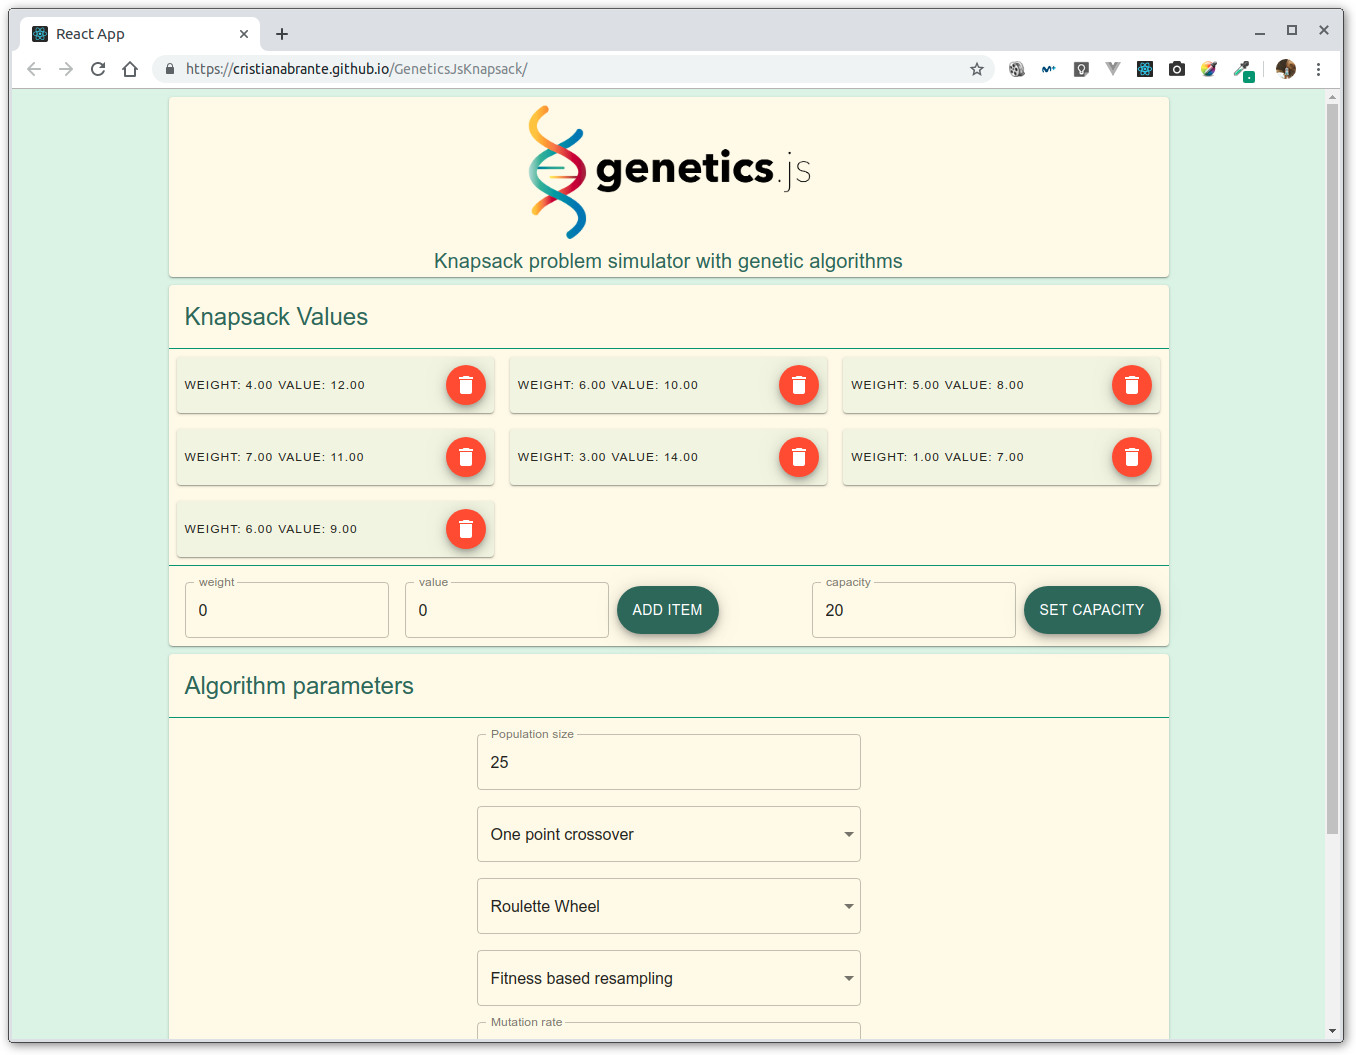
\includegraphics[scale=0.2]{mem/images/cap-5/knapsack-1.png}
    \caption{Pantalla principal de la aplicación web desarrollada}
    \label{fig:screenshot-1}
\end{figure}

En la parte central de la pantalla tendremos el formulario en el que se muestran los items que formarán parte de la mochila. Podremos introducir items y también eliminarlos, pudiendo a su vez establecer el peso y cantidad del item en cuestión. Además, en la parte derecha contamos con un campo de texto en el que podremos introducir la capacidad de la mochila. Cabe señalar que ambos formularios están verificados para impedir que se introduzcan valores erróneos. \\

El segundo formulario con el que nos encontramos es el de parámteros del algoritmo. En el podremos elegir cuales serán las operaciones que se aplicarán a la hora de ejecutar el algoritmo genético. Al igual que ocurría en el caso anterior, en este formulario también se ha llevado a cabo una verificación para evitar los valores erróneos. \\

Una vez pulsamos el boton \textbf{execute algorithm} de la parte inferior, la aplicación nos llevaría a una segunda pantalla en la que se mostraría la ejecución del algoritmo.

\begin{figure}[H]
    \centering
    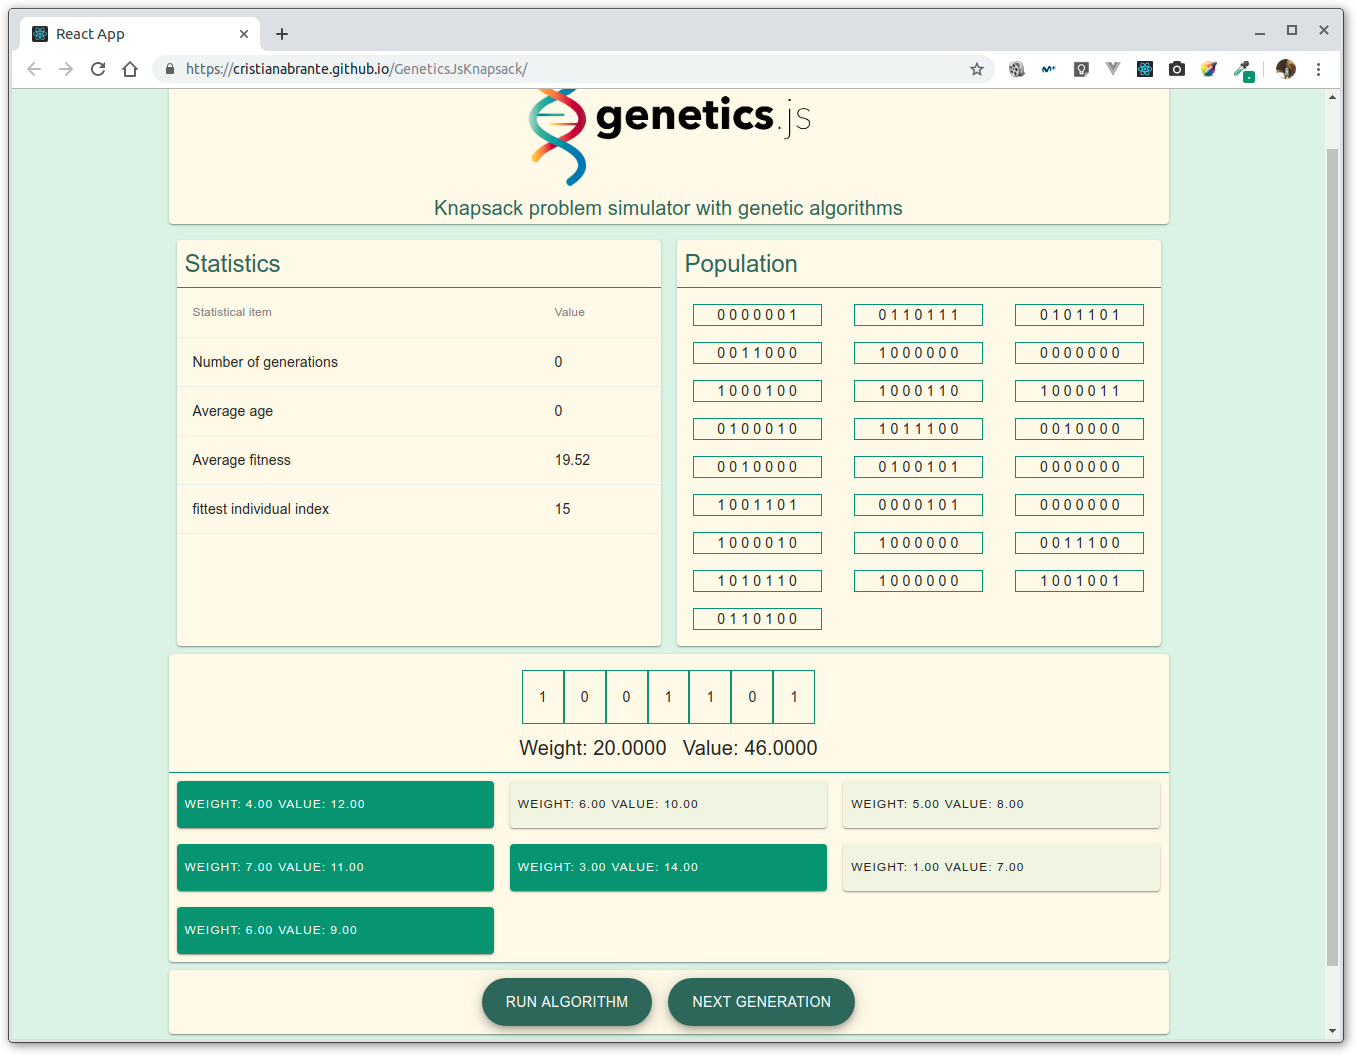
\includegraphics[scale=0.2]{mem/images/cap-5/knapsack-2.png}
    \caption{Pantalla de ejecución del algoritmo}
    \label{fig:screenshot-1}
\end{figure}

Esta pantalla está dividida en una serie de secciones diferentes. En la parte izquierda, contamos con una tabla en la que se muestran las estadísticas del algoritmo evolutivo, actualizadas durante la ejecución. Entre las estadísticas que se muestran encontramos: el número de generaciones, la edad media de los individuos, o el fitness medio de la población. \\

A la izquierda de este recuadro se puede ver una representación visual de la población, la cual se irá actualizando a medida que el algoritmo se ejecute. La visualización de este apartado es la que impide que se tengan tamaños de población muy grandes. \\

Finalmente y en la parte inferior, nos encontramos una representación del individuo con un mayor valor de fitness, indicando cuales son los items que ha escogido para introducir en la mochila, así como el peso y valor que tendrá dicha selección. \\

La ejecución del algoritmo se puede hacer de manera contínua, ejecutando de una sola vez el algoritmo hasta que se llegue a un máximo de generaciones, o también se puede hacer paso a paso, por si se quiere depurar el resultado. \\

El despliegue de esta aplicación se ha hecho en \textbf{GitHub pages}, y por tanto está disponible en este enlace: \url{https://cristianabrante.github.io/GeneticsJsKnapsack/}.
